\section{Related Work}

\begin{figure}[tb]
    \centering
    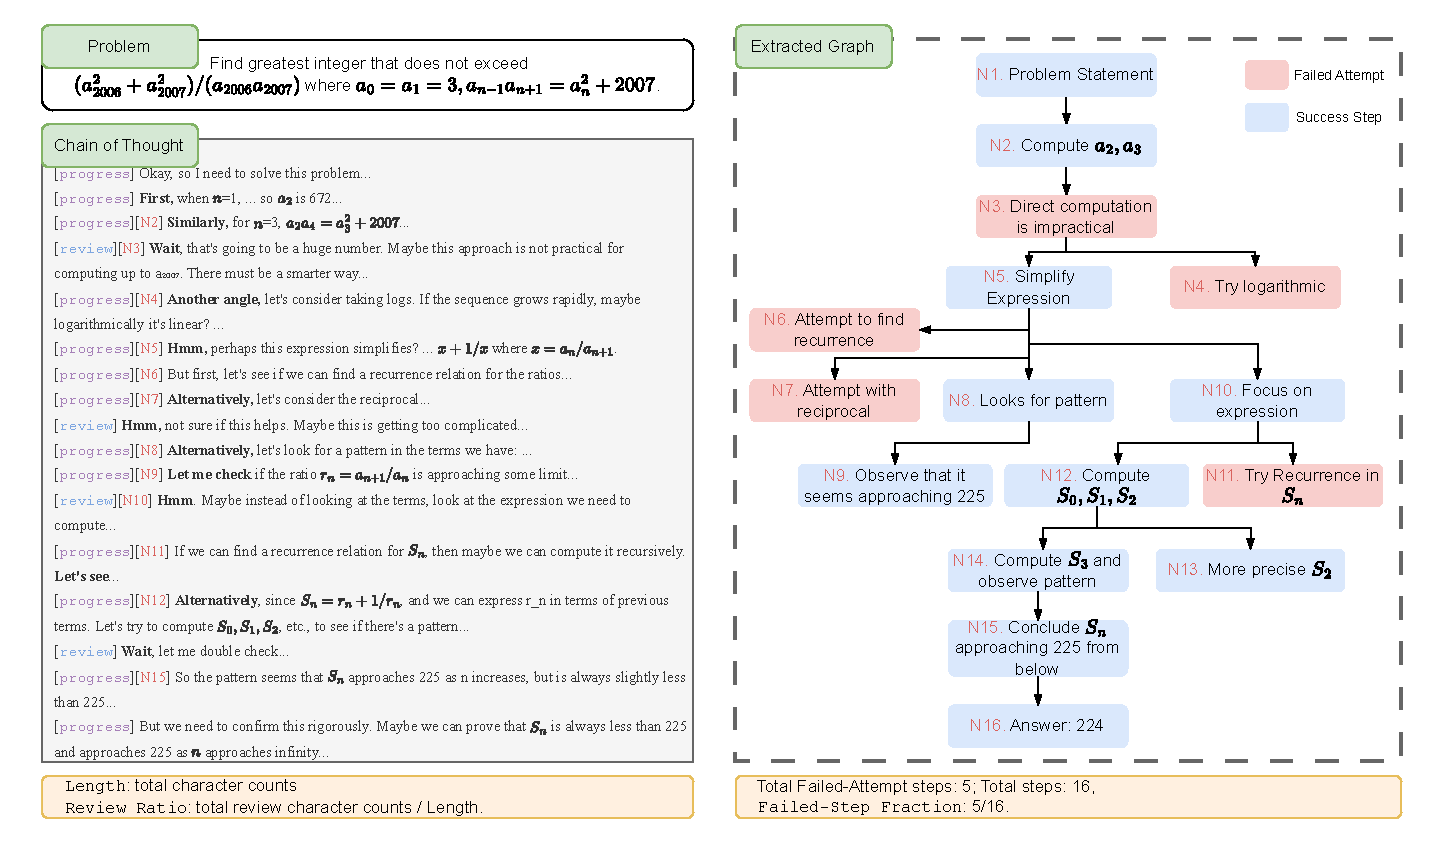
\includegraphics[width=1\linewidth]{final_figs/cot_teaser_2.pdf}
    \caption{\textbf{Example.} A chain-of-thought (left) with \Review annotations and the corresponding extracted reasoning graph (right). The CoT is segmented into semantic chunks (Section \ref{sec:lexical}), each labeled \texttt{Progress} or \texttt{Review}; from these labels we compute \Length and \rr. The right panel shows the extracted graph with nodes ($N_1:N_{16}$); red nodes denote failed attempts (Section \ref{sec:graphical}). Each node maps faithfully to a span in the CoT. Using this graph annotation, we measure \failedstep.}
    \label{fig:data_visualization}
\end{figure}

% Existing (concurrent) works either define metrics with human definition or with quantitative expressions. The metrics with human definition are typically measured with LLM as a judge technique. However, there is a lack of reliability analysis on whether the metric reliably measure the definition. \CZ{Not sure about the measuring of the previous sentence. In general, we want to answer: 1. what are good measure of reasoning trace quality that can be indicative for final model performance. 2. What are good factors to encourage or discourage to lead to better final model performance . 3. Bonus: See the measure of final answer accuracy quality aligns with human judgment quality. TBD if we want to get three. We may not do it but if there is insight, we can discuss
 % }

% Paper for short CoTs: 

% Direct metrics:

% Metrics based on reasoning graph:


% However, it is not clear on 

\paragraph{Scaling Test-Time Compute} \quad Large reasoning models (LRMs) increasingly rely on long, step-by-step CoT traces, reflecting a shift from scaling compute at training time to scaling at test time. This trend is exemplified by OpenAI's O1 series \citep{jaech2024openai} and DeepSeek R1 \citep{guo2025deepseek}, which often generate CoTs with tens of thousands of tokens before providing a final answer. As the number of tokens produced during inference grows, performance tends to improve, exhibiting characteristic test-time scaling behavior.

\yunzhen{Various research approaches have explored methods to achieve this scaling.} Among these, the S1 study \citep{muennighoff2025s1} appends \textit{wait} tokens to increase generation length, prompting the model to continue generating and review its prior reasoning. Follow-up works \citep{ringel2025learning, jurayj2025your} replace the fixed \textit{wait} token with learned "continue thinking" prompts, reporting larger gains. However, recent work has produced conflicting findings: \citet{wang2025wait} show that suppressing \textit{wait} can preserve accuracy while reducing length; \citet{ghosal2025does, marjanovic2025deepseek, wu2025s} observe that continually adding \textit{wait} initially helps but ultimately degrades performance; and \citet{wu2025more} provide evidence that longer CoTs are not always better. Furthermore, several results are restricted to small model sets, leaving unclear whether different LRMs exhibit similar behavior. Motivated by these mixed results, we conduct a systematic study across 10 models to understand how \Length and \Review behaviors generally affect reasoning.

% \textbf{Scaling Test-Time Compute as S1.} \quad Among early approaches, the S1 study \citep{muennighoff2025s1} appends \textit{wait} token to increase generation length. The model is prompted to continue generating and review its prior reasoning, and shows improved performance. Follow-up works \citep{ringel2025learning, jurayj2025your} replace the fixed \textit{wait} token with learned “continue thinking” prompts or “Is That Your Final Answer?” tokens, reporting larger gains and improved calibration. More recently, several works reassess these interventions: \citet{wang2025wait} show that suppressing the probability of generating \textit{wait} can preserve or even improve accuracy while substantially reducing length; \citet{ghosal2025does, marjanovic2025deepseek, wu2025s} observe that continually adding \textit{wait} initially increases performance but ultimately degrades it beyond a threshold; and \citet{wu2025more} provide empirical and theoretical evidence that longer CoTs are not always better. Furthermore, several results are restricted to a small set of models, so it remains unclear whether different LRMs exhibit similar behavior. Motivated by these mixed results, we conduct a systematic study over 10 models to understand how generally \Length and \Review behaviors affect the reasoning. 

\paragraph{Extracting Reasoning Structure} \quad \yunzhen{To understand the structural properties of reasoning traces, recent work \citep{jiang2025makes, minegishi2025topology} has explored representing CoT reasoning as graphs, where nodes capture reasoning steps and edges represent logical dependencies or flow between steps.}  Extracting a faithful reasoning graph from an existing CoT is challenging, and only a few recent or concurrent papers attempt it. \citet{jiang2025makes} propose a six-round prompt scaffold for summarization, segmentation, and node assignment to extract the graph. \citet{minegishi2025topology} instead leverage internal representations: they aggregate sentence-level hidden embeddings, cluster them with $k$-means to form nodes, and connect nodes in the order visited. By contrast, we directly elicit graphs from the model, relying on Graphviz extraction capabilities learned in pretraining and avoiding both multi-call scaffolding and sentence-level embeddings.

\paragraph{Characterizing Effective Reasoning} \yunzhen{Understanding what makes reasoning effective is fundamental to improving LRMs.} \citet{guo2025deepseek} showcases an “aha moment,” in which the model reviews its previous steps. Subsequent work identifies cognitive behaviors, such as verification and backtracking, as important for reasoning \citep{gandhi2025cognitive, hu2025beyond}. However, these behaviors are difficult to measure reliably and previous studies often construct them on synthetic tasks. At the graph level, \citet{jiang2025makes, minegishi2025topology} analyze reasoning-tree structure and find these features to matter; \citet{wu2025knowledge} examines knowledge correctness and information gain. Our primary analysis centers on \Length, \rr, and graph-based \fsf; additional complementary metrics are provided in Appendices \ref{appendix:graph} and \ref{append:further}.



% operationalize these ideas by (i) measuring \(\rr\) to quantify review behaviors, (ii) extracting graph-level features, and (iii) incorporating complementary metrics such as motivation level.


% \textbf{What characterize Effective Reasoning?} This is a foundamental question to reasoning. R1 paper \citep{guo2025deepseek} showcase the example of 'aha moment' that the model review its prior steps. Following paper further identify cognitive behaviors \citep{gandhi2025cognitive, hu2025beyond} including verification and backtracking that is important for reasoning. It is generally hard to measure these behavoirs and prior work only perform it for synthetic task. \citet{jiang2025makes, minegishi2025topology} looks at reasoning graph level and find these features to be important. \citet{wu2025knowledge} check the knowledge correctness, and information gain. In our work, we measure \rr to quantify the review hebaviors, extract graph features, and also include other metrics like motivation level and 


% . In fact, on benchmarks like the MATH dataset and LiveCodeBench, selecting answers via the reasoning-tree classifier improved accuracy by up to 10% over baseline selection methods
% arxiv.org
% % . Complementary to this, Cao (2024) introduces GraphReason, a verification approach that merges multiple distinct CoT solutions into a global reasoning graph
% arxiv.org
% . Here, each node represents a shared intermediate step and edges capture logical connections between steps across different candidate solutions. A trained Reasoning Graph Verifier then judges the correctness of an answer by analyzing the topology of this graph
% arxiv.org
% . This method achieved state-of-the-art performance on math word problems, outperforming prior self-consistency and stepwise verifiers – for instance, boosting accuracy on GSM8K from 72.7% to 85.7% (a 13% absolute gain)
% ar5iv.org
% . In summary, across domains such as mathematical reasoning, multi-hop question answering, and beyond, researchers have begun to extract explicit graph structures from LLM-generated reasoning traces – from trees that reveal the latent hierarchy of thoughts to more general graphs that fuse and verify multiple reasoning paths – in order to improve transparency and enhance problem-solving accuracy
% ar5iv.labs.arxiv.org
% arxiv.org
% . Each of these approaches treats the model’s free-form rationale as a structured graph, enabling deeper analysis of the reasoning process and often yielding superior results on complex reasoning benchmarks.